\documentclass{article}
\usepackage{listings}
\usepackage{graphicx}
\usepackage{hyperref}
\lstset{
   basicstyle=\scriptsize\ttfamily,
   numbers=left,
   frame=single,
   breaklines=true,
   breakautoindent=true,
   postbreak={\mbox{$\hookrightarrow$}},
   literate={ä}{{\"a}}1 {ö}{{\"o}}1 {ü}{{\"u}}1 {ß}{{\ss}}1 {Ä}{{\"A}}1 {Ö}{{\"O}}1 {Ü}{{\"U}}1}

\hypersetup{
  colorlinks=false,
  pdfborder={0 0 0},
}
\setlength{\topmargin}{1.5cm}
\setlength{\headheight}{12pt}
\setlength{\headsep}{20pt}
\setlength{\topskip}{12pt}
\setlength{\evensidemargin}{0pt}
\setlength{\oddsidemargin}{10mm}
\setlength{\textheight}{230mm}
\setlength{\textwidth}{150mm}
\setlength{\voffset}{-2cm}
\setlength{\parindent}{0pt}
\setlength{\parskip}{6pt}

%opening
\title{Systemsicherheit - 4. Übung}
\author{Dennis Rotärmel, Niklas Entschladen, Tobias Ratajczyk, Gruppe Q}

\begin{document}
\maketitle
	
\newpage
\thispagestyle{empty}
\section{Aufgabe 1: Control-Flow Graph (CFG)}
\begin{figure}[h]
	\centering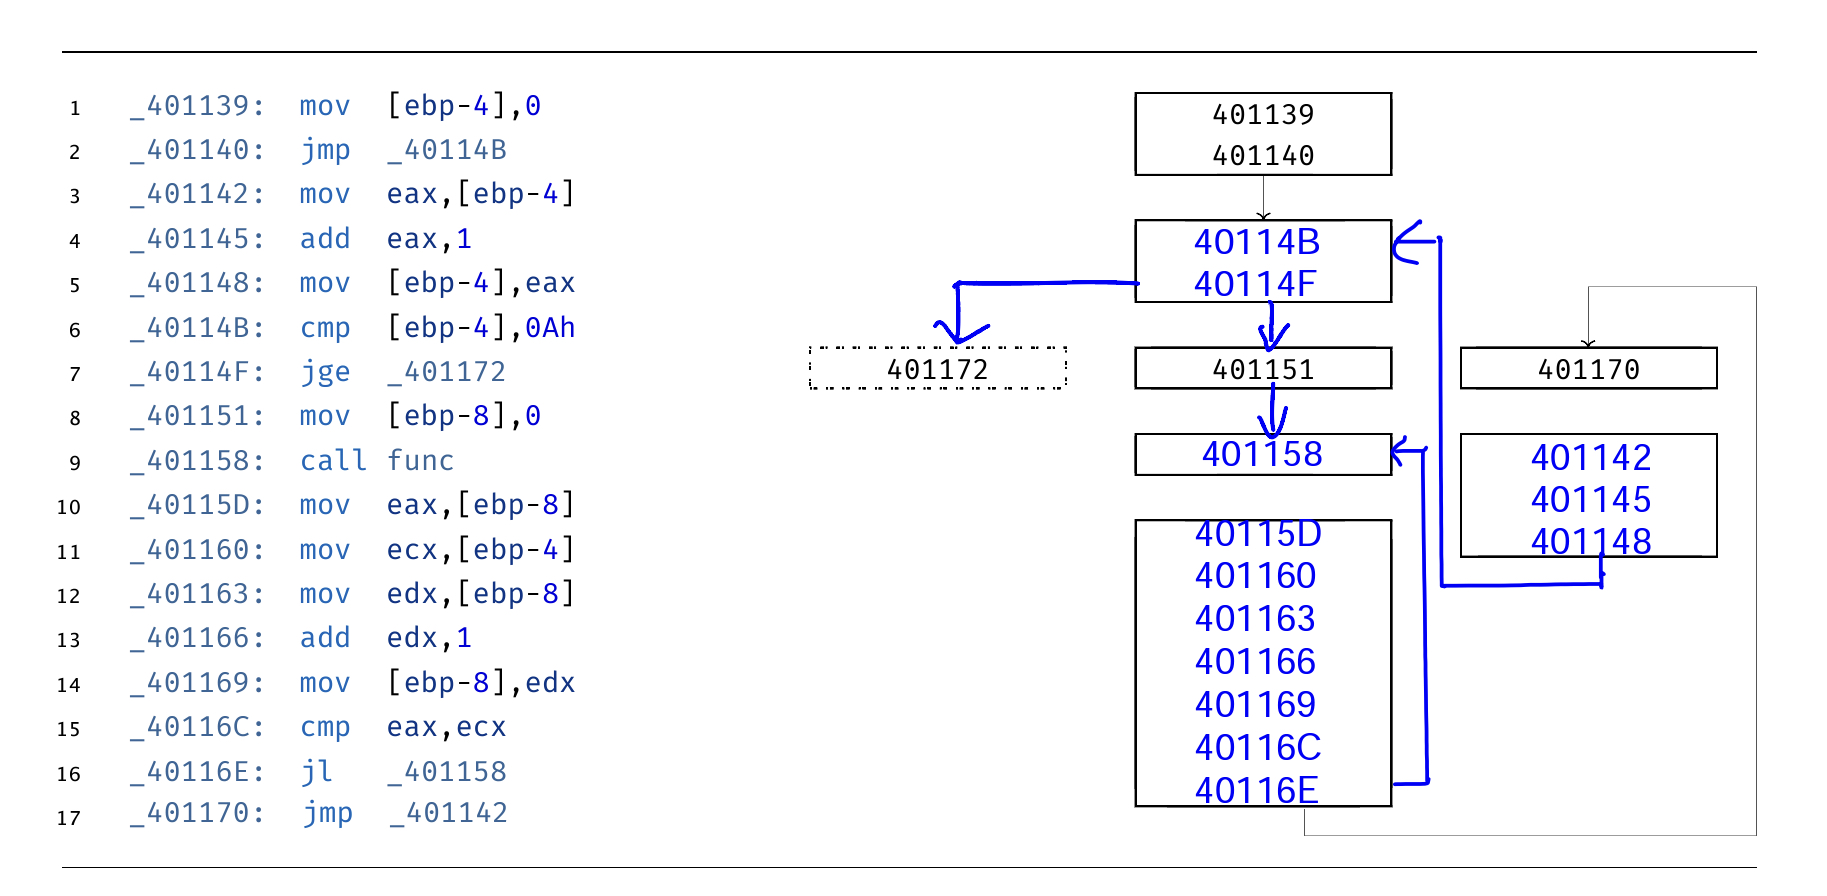
\includegraphics[width=1.0\textwidth]{images/1a.jpeg}
	\caption{Control-Flow Graph}
\end{figure}
\pagebreak
\section{Aufgabe 2: Data Execution Prevention (DEP)}
\subsection{a)}
\begin{figure}[h]
\centering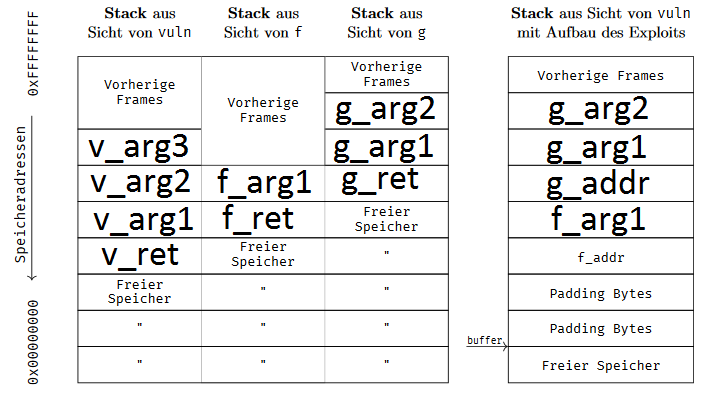
\includegraphics[width=1.0\textwidth]{images/2a_stacks.png}
\caption{Control-Flow Graph}
\end{figure}
Sobald eine Funktion returnt, wird die nächste Instruktion im Stack ausgeführt. Dies stellt in unserem Fall den Sprung zu einer neuen Funktion dar, welche für einen Code Reuse Angriff benutzt werden.\\
Es wäre ein Problem, wenn die Funktion \verb|f| einen Parameter mehr erwartet, da sie dann die Adresse der Funktion \verb|g| als zweiten Parameter annimmt, während der erste Parameter der Funktion \verb|g| fälschlicherweise die Adresse dieser Funktion darstellt. Für die Funktion \verb|g| gilt nicht diese Einschränkung, da die Funktion \verb|g| die letzte Library-Funktion der Chain darstellt. Die vorigen Stackframes haben keinen Einfluss auf die Code Reuse Attack.\\
Das Problem, wenn wir nach Funktion \verb|f| und \verb|g| noch eine weitere Funktion aufrufen wollen, liegt darin dass der Inhalt des vorigen Stackframes korrumpiert wird, sodass das Programm abstürzen könnte.
\subsection{b)}

\section{Aufgabe 3: Stack Canaries}
	
\section{Aufgabe 4: Address Space Layout Randomization (ASLR)}
	
\end{document}